\chapter{Engenharia de Software}\label{chap:software}
\begin{quote}\normalfont\itshape\vspace*{-2\baselineskip}
% Neste capiulo serão descritas as fases de especificação e projeto do sistema. Ainda nesse capítulo são apresentadas as ferramentas e a arquitetura do sistema, dando uma visão geral do que foi desenvolvido.
\end{quote}

% Engenharia de Software pode ser definida como:
% \begin{citacao}[english]
% 1. the systematic application of scientific and technological knowledge, methods, and experience to the design,
% implementation, testing, and documentation of software [...]  2. the application
% of a systematic, disciplined, quantifiable approach to the development, operation,
% and maintenance of software; that is, the application of engineering to software \cite{IEEE2010}.
% \end{citacao}
%
% \begin{figure}[!b]
%   \centering
%   \caption{Engenharia de Software - uma tecnologia em camadas}
%   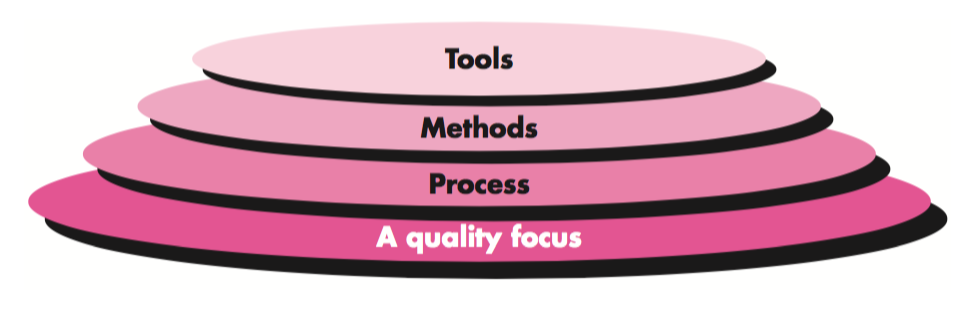
\includegraphics[scale=0.33]{imagens/desenv_engsoft2}
%   \label{fig:desen_engsoft}
%   \fonte{\cite{Pressman2009}}
% \end{figure}
%
% A engenharia de software deve ter foco na qualidade, que apoia as outras camadas
% dessa tecnologia, que são as camadas de processo, métodos e ferramentas \autoref{fig:desen_engsoft}.
% A camada de processo define um conjunto de atividades ou um arcabouço que tem
% como finalidade garantir a efetiva utilização da tecnologia engenharia de software, que dessa forma
% leva à produção de um software. Os detalhes de como fazer o software pertencem
% a camada de métodos. Os métodos da engenharia de software incluem tarefas de planejamento
% e estimativa de software, análise de requisitos, modelagem de projeto, codificação,
% testes e manutenção. As ferramentas de engenharia de software auxiliam as camadas de
% processo e métodos, com ferramentas automatizadas, que por sua vez, quando integradas,
% é estabelecido um suporte ao desenvolvimento de software chamado CASE\nomenclature{CASE}{Computer Aided Software Engineering} -
% \textit{Computer Aided Software Engineering} \cite{Pressman2009, Sommerville2006}.
%
% Entre o conjunto de atividades definidas pela camada de processo, quatro são
% fundamentais, a saber, especificação de software, projeto e implementação de
% software, validação de software e evolução de software. Especificação de software
% ou engenharia de requisitos é uma fase importante e crítica do processo de engenharia
% de software. Importante porque é uma análise de requisitos bem feita que possibilitará
% atendar as demandas dos usuários. Crítica porque um sistema mal especificado, pode até ser
% bem projetado e construído, mas não vai atender as necessidades dos usuários.
% Em seguida, na fase de projeto e implementação os requisitos são projetados e programados,
% tendo como resultado um sistema executável. Depois, o software deve ser verificado
% para mostrar que atende às demandas dos usuários (validação do software). Finalmente,
% na fase de evolução de software, o mesmo é modificado devido às mudanças
% de requisitos e às necessidades dos usuários.
%
% \subsection{Especificação do Sistema}
% Nessa primeira etapa do projeto, foi utilizada a ferramenta \textit{Astah Community} \cite{astah2016}
% para a criação de documentação em linguagem de modelagem unificada (UML)\nomenclature{UML}{Unified Modeling Language}. Os diagramas
% de casos de uso UML são largamente utilizados para especificação de requisitos \cite{Sommerville2006}.
% A \autoref{fig:usecases} exemplifica os casos de uso do sistema, fornecendo uma
% visão geral do mesmo.
%
% \begin{figure}[!htb]
%   \centering
%   \caption{Diagrama de Caso de Uso: Visão geral do sistema}
%   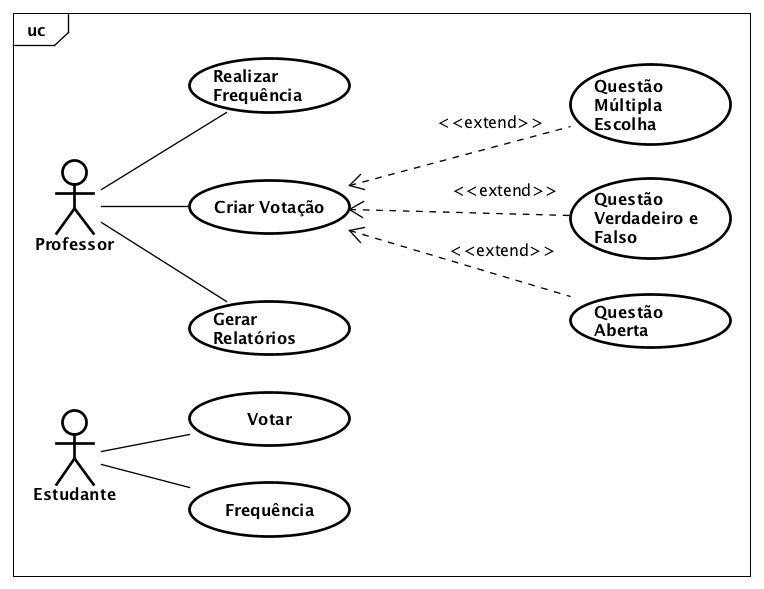
\includegraphics[width=.75\textwidth]{imagens/casodeuso}
%   \fonte{Elaborado pelo autor}
%   \label{fig:usecases}
% \end{figure}
%
% \subsection{Projeto e Implementação}
% O diagrama de implantação UML ou \textit{deployment diagram} mostra o \textit{hardware}
% do sistema ou elementos de processamento, os componentes de software instalados
% no \textit{hardware} e o \textit{middleware} usado para conectar os diferentes
% nós do sistema \cite{Pressman2009}. A \autoref{fig:deployment_diagram} mostra
% o diagrama de implantação do sistema que será desenvolvido. É possível observar
% uma solução simples, mas que faz uso de soluções \textit{open-source} e de
% qualidade reconhecida como será descrito a seguir.
%
% \subsubsection{Plataforma}
%
% \begin{figure}[!b]
%   \centering
%   \caption{Diagrama de Implantação do sistema}
%   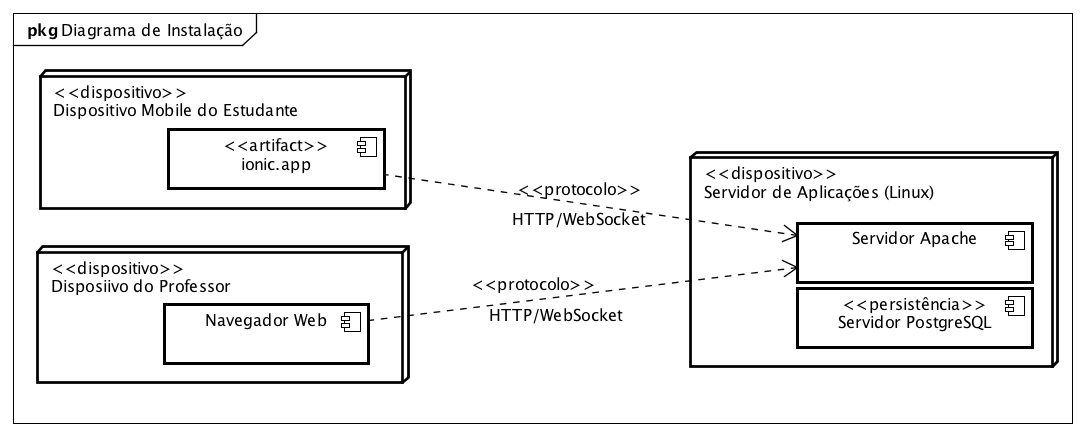
\includegraphics[width=1\textwidth]{imagens/deployment_diagram}
%   \fonte{Elaborado pelo autor}
%   \label{fig:deployment_diagram}
% \end{figure}
%
% \begin{description}
%   \item[Servidor HTTP Apache]
%   o Servidor HTTP\nomenclature{HTTP}{Hypertext Transfer Protocol} Apache (``httpd'') foi lançado em 1995 e desde abril de 1996 é o
%   servidor web \textit{open-source} mais popular do mundo \cite{apache2016}.
%   Segundo \citeonline{W3Techs2016} o Apache é usado por 51,3\% dos sites ativos no mundo.
%
%   \item[PostgreSQL] sistema gerenciador de banco de dados objeto relacional (SGBDOR).
%   Entre os SGBDORs\nomenclature{SGBDORs}{Sistema Gerenciador de Banco de Dados Objeto Relacional}
%   \textit{open-source} mais avançados, totalmente compatível com
%   o padrão ANSI-SQL:2008\nomenclature{ANSI-SQL}{American National Standards Institute - Structured Query Language},
%   com recursos de integridade de dados includindo chaves
%   primárias compostas, chave estrangeira, restrições \textit{check, unique, not null},
%   gatilhos (\textit{triggers}), visões (\textit{views}), \textit{storage procedures}
%   e recursos avançados como colunas de auto-incremento por exemplo.
%   O PostgreSQL é distribuído sobre a licença permissiva MIT \cite{postgree2016}.
%
%   \item[Python] uma das linguagens de programação mais populares do mundo,
%   figurando entre as 5 linguagens mais utilizadas \cite{TIOBE2016, RedMonk2016, PYPL2016}.
%   A escolha pela tecnologia Python como linguagem de programação se deu principalmente
%   porque um dos principais \textit{frameworks} para o desenvolvimento web \textit{Django} \cite{Django2016},
%   é escrito em Python. O \textit{Django} conta com mapeador objeto-relacional,
%   interface de administração automática, URL's\nomenclature{URL}{Uniform Resource Identifier} elegantes, sistema de templates e
%   sistema de cache \cite{Django2016}.
%
%   \item[Ionic] é um \textit{framework open-source} para o desenvolvimento de aplicativos
%   híbridos utilizando tecnologias web como HTML\nomenclature{HTML}{HyperText Markup Language},
%   CSS\nomenclature{CSS}{Cascading Style Sheets} e JavaScript otimizadas
%   para dispositivos móveis, com código fonte sobre a licença MIT\nomenclature{MIT}{Massachusetts Institute of Technology} \cite{ionic2016}.
%   Uma das principais vantagens do desenvolvimento de aplicativos híbridos é que com
%   apenas um código base é possível criar aplicativos para várias plataformas como
%   iOS, Android e Windows Phone, que aliás foi uma das razões que fez o Moodle
%   usar o Ionic como \textit{framework} para o desenvolvimento do \textit{Moodle Mobile 2} \cite{moodle2016}.
%
%   \item[WebSocket] é um protocolo que possibilita abrir um canal interativo de comunicação
%   entre o navegador e o servidor. Na verdade, esse canal é bidirecional (\textit{full-duplex})
%   que utiliza apenas um soquete TCP\nomenclature{TCP}{Transmission Control Protocol} \cite{websocket2016}. A tecnologia \textit{WebSocket} será usada
%   para permitir votação e controle de frequência em tempo-real.
% \end{description}

\clearpage
\section{Engenharia de Software}

Engenharia de Software pode ser definida como:
\begin{citacao}[english]
1. the systematic application of scientific and technological knowledge, methods, and experience to the design,
implementation, testing, and documentation of software [...]  2. the application
of a systematic, disciplined, quantifiable approach to the development, operation,
and maintenance of software; that is, the application of engineering to software \cite{IEEE2010}.
\end{citacao}

A engenharia de software deve ter foco na qualidade, que apoia as outras camadas
dessa tecnologia, que são as camadas de processo, métodos e ferramentas \autoref{fig:desen_engsoft}.
A camada de processo define um conjunto de atividades ou um arcabouço que tem
como finalidade garantir a efetiva utilização da tecnologia engenharia de software, que então
leva à produção de um software. Os detalhes de como fazer o software pertencem
a camada de métodos. Os métodos da enghenharia de software incluem tarefas de planejamento
e estimativa de software, análise de requisitos, modelagem de projeto, codificação,
testes e manutenção. As ferramentas de engenharia de software auxiliam as camadas de
processo e métodos, com ferramentas automatizadas, que por sua vez, quando integradas,
é estabelecido um suporte ao desenvolvimento de software chamado CASE -
\textit{Computer Aided Software Engineering} \cite{Pressman2009, Sommerville2006}.

\begin{figure}[b]
  \centering
  \caption{Engenharia de Software - uma tecnologia em camadas}
  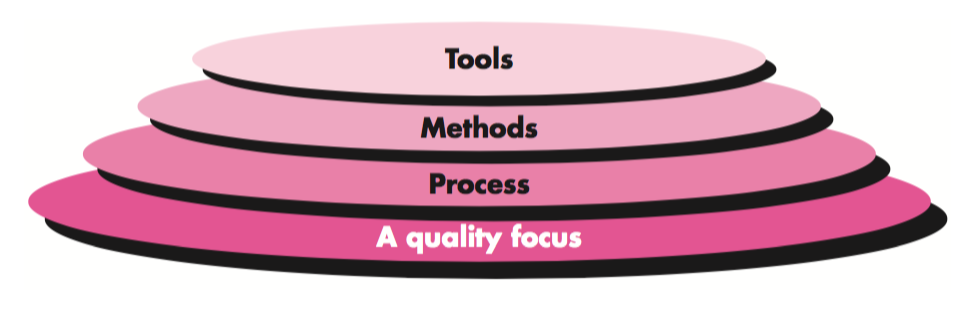
\includegraphics[scale=0.3]{imagens/desenv_engsoft2}
  \label{fig:desen_engsoft}
  \fonte{\cite{Pressman2009}}
\end{figure}

Entre o conjunto de atividades definidas pela camada de processo, quatro são
fundamentais, a saber, especificação de software, projeto e implementação de
software, validação de software e evolução de software. Especificação de software
ou engenharia de requisitos é uma fase importante e crítica do processo de engenharia
de software. Importante porque é uma análise de requisitos bem feita que possibilitará
atendar as demandas dos usuários. Crítica porque um sistema mal especificado, pode até ser
bem projetado e construído, mas não vai atender as necessidades dos usuários.
Em seguida, na fase de projeto e implementação os requisitos são projetados e programados,
tendo como resultado um sistema executável. Depois, o software deve ser verificado
para mostrar que atende às demandas dos usuários (validação do software). Finalmente,
na fase de evolução de software, o software é modificado devido às mudanças
de requisitos e às necessidades dos usuários.

